 \documentclass{article}
    \usepackage{amsmath}
    \usepackage[utf8]{inputenc}
    \usepackage[english]{babel}
    \usepackage{color}
    \usepackage{graphicx}
    \usepackage{enumitem}
    \hyphenpenalty=10000
    \exhyphenpenalty=10000
    % \usepackage[T1]{fontenc}
    % \usepackage{geometry}
    \usepackage[top = 2cm, bottom = 2cm]{geometry}
    
    \usepackage[familydefault,light]{Chivo} 
    \usepackage[T1]{fontenc}
    
    \setlength{\parindent}{4em}
    \setlength{\parskip}{2em}
\renewcommand{\baselinestretch}{1.5}
    \usepackage{graphicx}
    
    \title{COL 783 \\ Assignment 2}
    \author{Rajbir Malik \\ 2017CS10416}
    
    \begin{document}
    
    \maketitle

%  Starting page
% -------------------------------------------------------
% -------------------------------------------------------
    \begin{center}
    \Large{\underline{\textbf{Denoising and Deblurring}}}
    \end{center}
    \subsection*{Overview}
    In this assignment, we were asked to understand and try various operations to recover an image after having been corrupted by nose and blurring.\\ 
    We progressively managed to get better restoration by first trying fixing with basic \textbf{mean} and \textbf{median filters}, which are innately unaware of the features in the image. \\ 
    Then we moved onto intelligent restorations process, in this case \textbf{edge preserving denoisers}. I chose to implement \underline{\textbf{Total variation denoising (Rudin et al., 1992)}}. \\
    Then we referred to \textit{Weiner Filtering} for \textit{deblurring} of various images. We tried with \textit{different noise levels} and \textit{different original image estimates.} \\
    Finally, we put things to practice, working with real life images and trying to bring them to closest possible restoration. \\
    The assignment was divided in 4 different sections, each of which are discussed separately, as followed.
    
% -------------------------------------------------------
% -------------------------------------------------------
% Topic I
    \pagebreak
    \subsection*{Basic Denoising}
    Here we were asked to add noise to the images provided and then try to denoise with various filters. \texttt{Gaussian} and \texttt{Salt/Pepper} noises were used and restoration filters in check were the \textbf{mean} and the \textbf{median filter}.\\
    Following images were provided.
    
    \begin{figure}[!htb]
    \minipage{0.45\textwidth}
      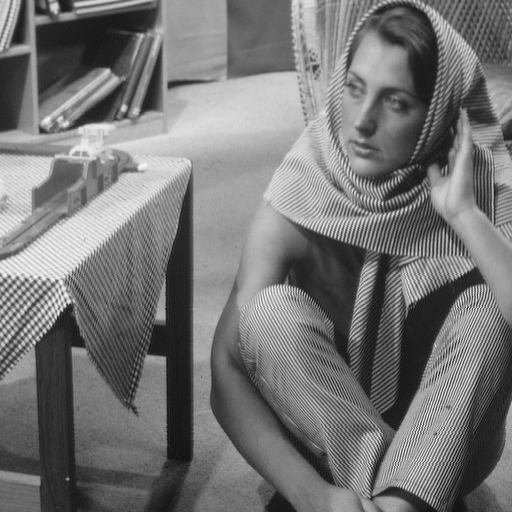
\includegraphics[scale=.35]{../images/barbara.png}
      \caption{Barbara}
    \endminipage \hfill
    \minipage{0.45\textwidth}
      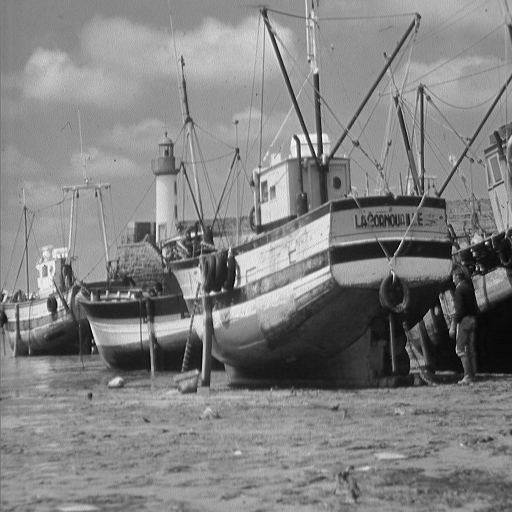
\includegraphics[scale=1.55]{../images/boat.png}
      \caption{Boat}
    \endminipage
    \end{figure}
    
    \phantom{}
    
    \begin{figure}[!htb]
    \minipage{0.45\textwidth}
      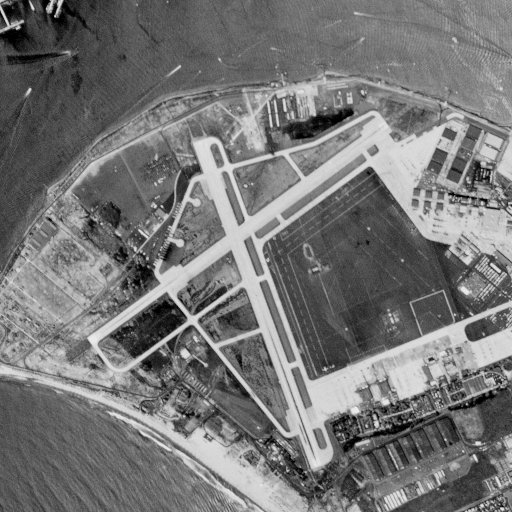
\includegraphics[scale=1.4]{../images/sandiego.png}
      \caption{Sandiego}
    \endminipage \hfill
    \minipage{0.45\textwidth}
      
\includegraphics[scale=.35]{../images/shepplogan.png}
      \caption{Shepplogan}
    \endminipage
    \end{figure}
    \pagebreak
    
% -------------------------------------------------------
% -------------------------------------------------------
% Barbara
% -------------------------------------------------------
% Gaussian
    \subsubsection*{Barbara (Gaussian)}
    
%   Image
    \begin{figure}[!htb]
    \begin{center}
     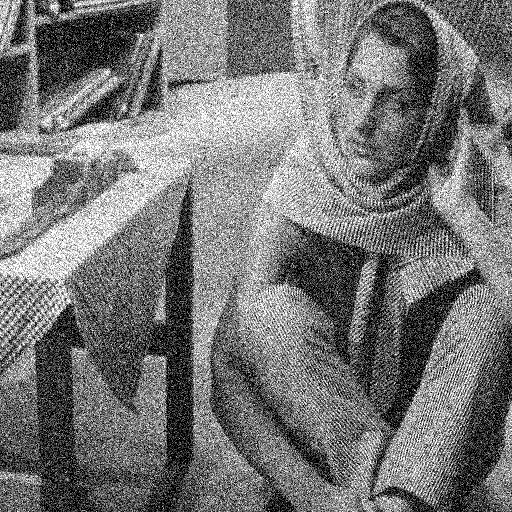
\includegraphics[scale=.3]{./basic_denoising/barbara/gaussian.png}
     \caption{Gaussian Noise}
    \end{center}
    \end{figure}
    
%   Mean Filter
    \begin{figure}[!htb]
    \minipage{0.45\textwidth}
      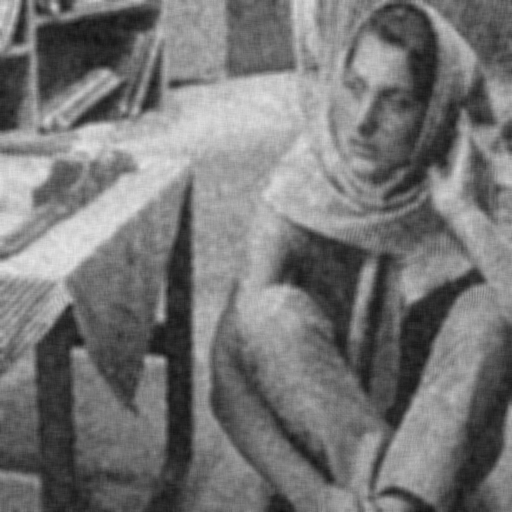
\includegraphics[scale=0.3]{./basic_denoising/barbara/average_best_gaussian.png}
      \caption{Best PSNR image}
    \endminipage \hfill
    \minipage{0.45\textwidth}
      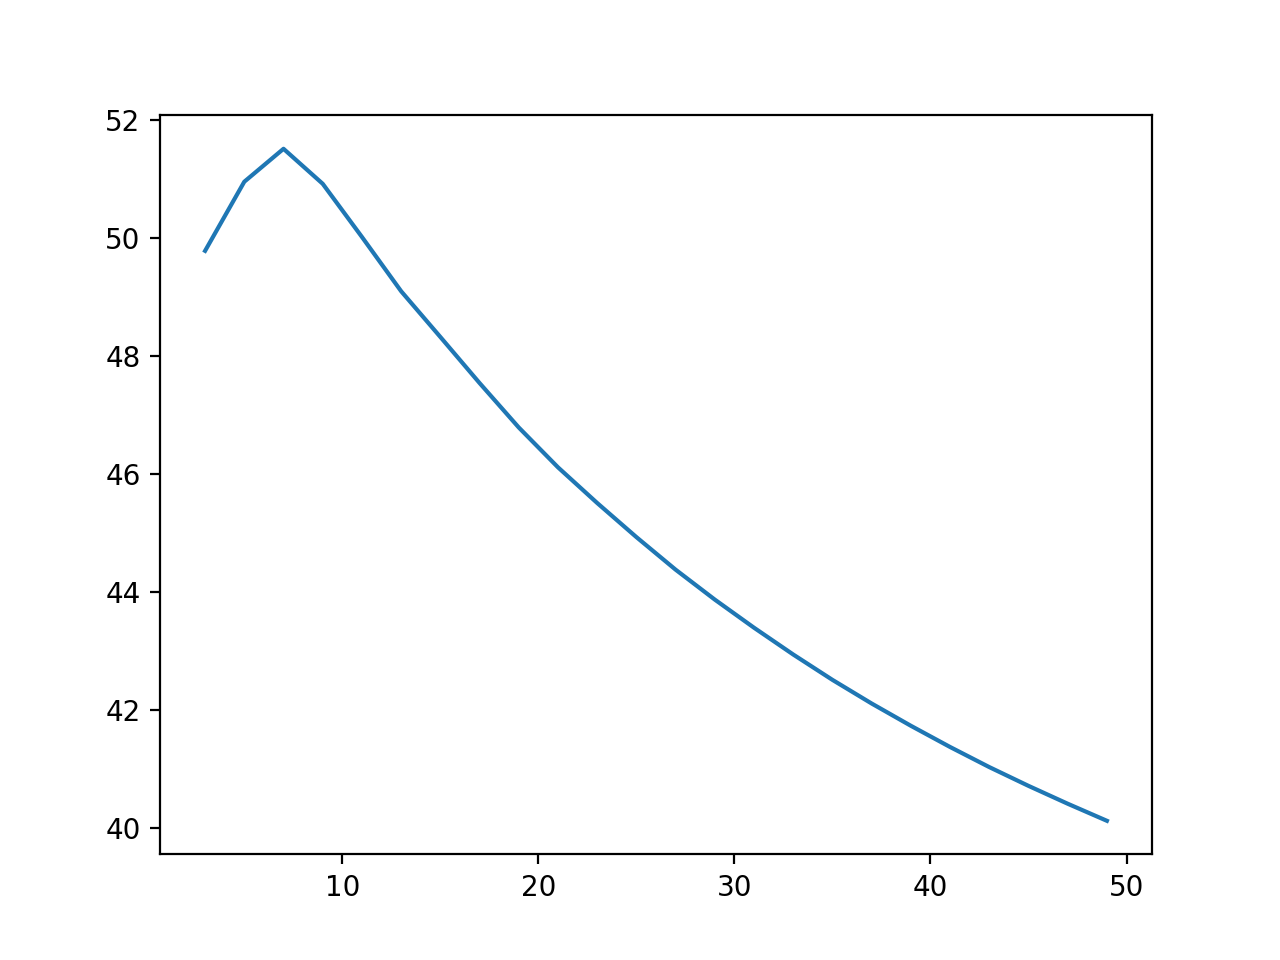
\includegraphics[scale=.45]{./basic_denoising/barbara/average_psnr_gaussian.png}
      \caption{PSNR vs filter size}
    \endminipage
    \end{figure}
    
%   Median Filter
    \begin{figure}[!htb]
    \minipage{0.45\textwidth}
      
\includegraphics[scale=0.3]{./basic_denoising/barbara/median_best_gaussian.png}
      \caption{Best PSNR image}
    \endminipage \hfill
    \minipage{0.45\textwidth}
      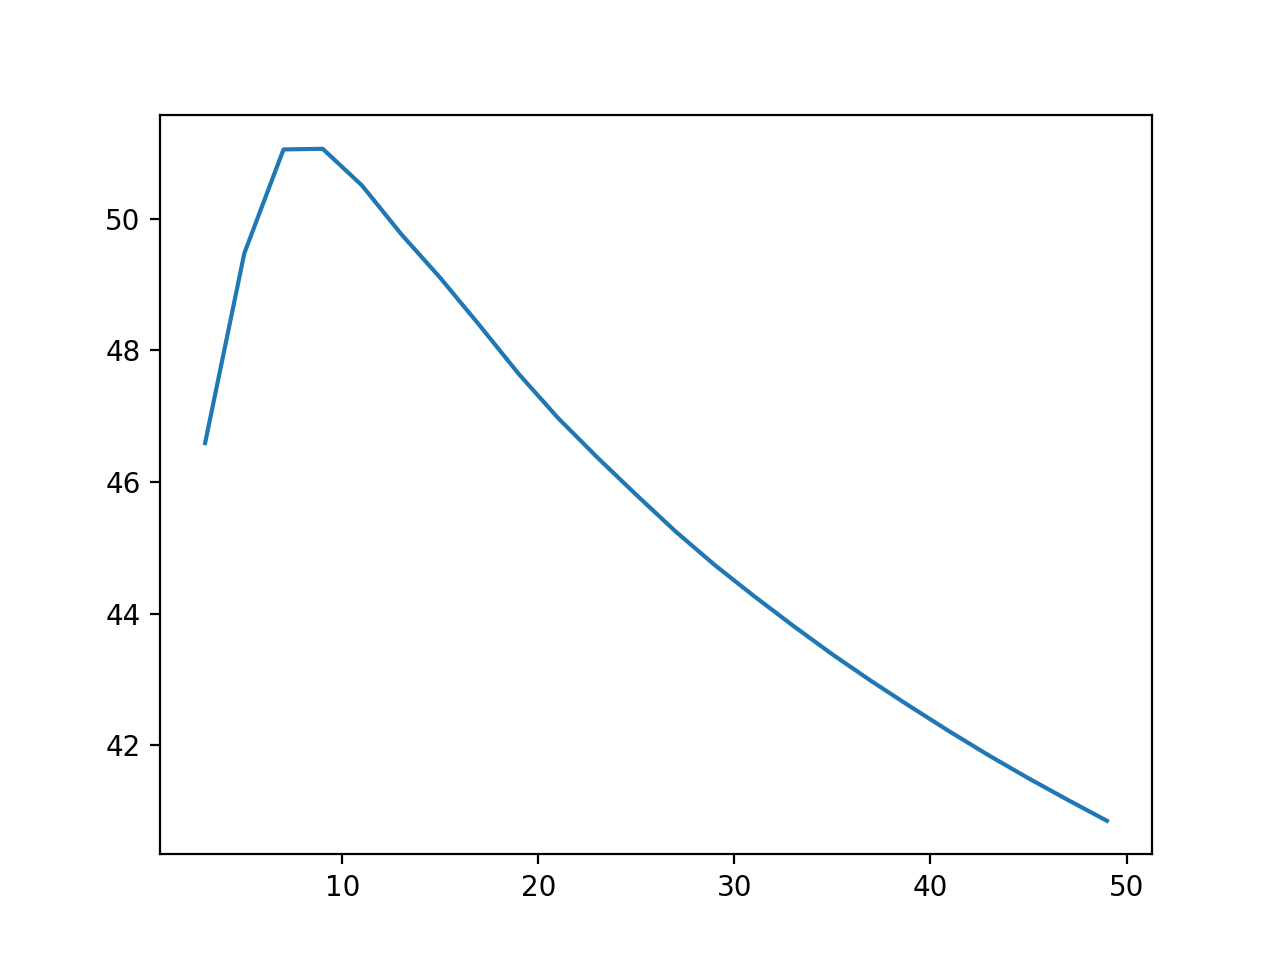
\includegraphics[scale=.45]{./basic_denoising/barbara/median_psnr_gaussian.png}
      \caption{PSNR vs filter size}
    \endminipage
    \end{figure}
    \pagebreak
% -------------------------------------------------------
% Salt\Pepper
    \subsubsection*{Barbara (Salt/Pepper)}
    
%   Image
    \begin{figure}[!htb]
    \begin{center}
     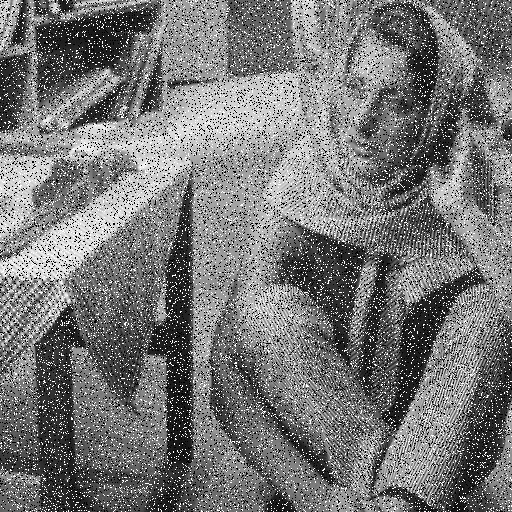
\includegraphics[scale=.3]{./basic_denoising/barbara/sp.png}
     \caption{Salt/Pepper Noise}
    \end{center}
    \end{figure}
    
%   Mean Filter
    \begin{figure}[!htb]
    \minipage{0.45\textwidth}
      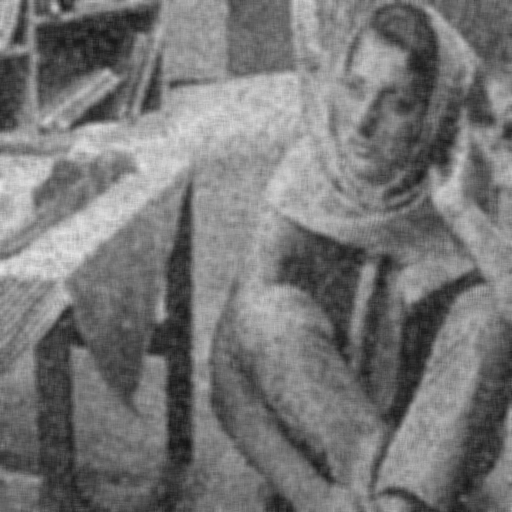
\includegraphics[scale=0.3]{./basic_denoising/barbara/average_best_sp.png}
      \caption{Best PSNR image}
    \endminipage \hfill
    \minipage{0.45\textwidth}
      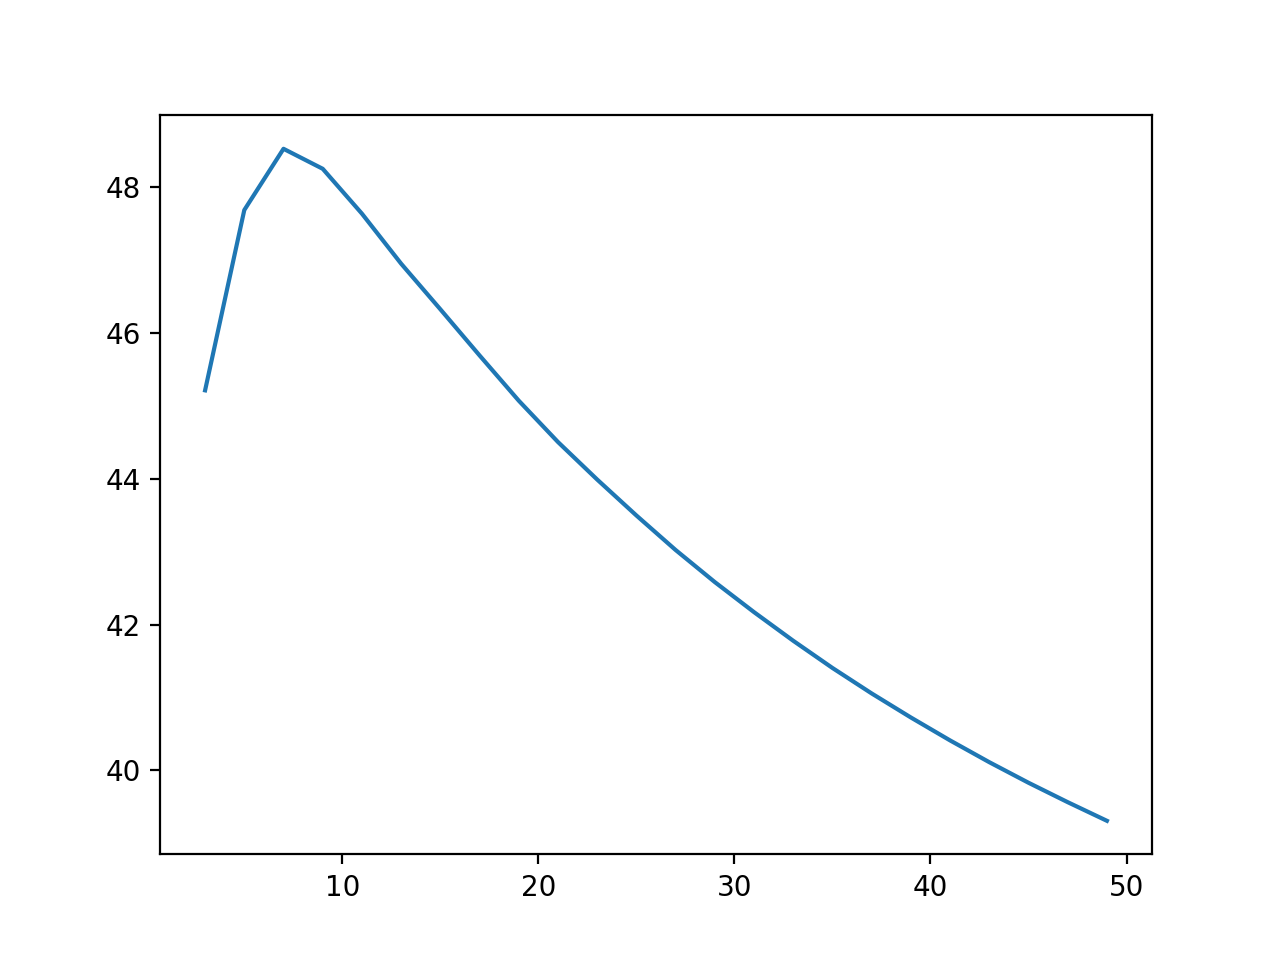
\includegraphics[scale=.45]{./basic_denoising/barbara/average_psnr_sp.png}
      \caption{PSNR vs filter size}
    \endminipage
    \end{figure}
    
%   Median Filter
    \begin{figure}[!htb]
    \minipage{0.45\textwidth}
      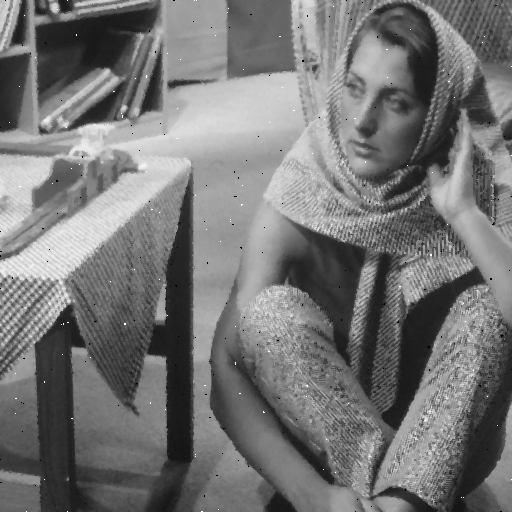
\includegraphics[scale=0.3]{./basic_denoising/barbara/median_best_sp.png}
      \caption{Best PSNR image}
    \endminipage \hfill
    \minipage{0.45\textwidth}
      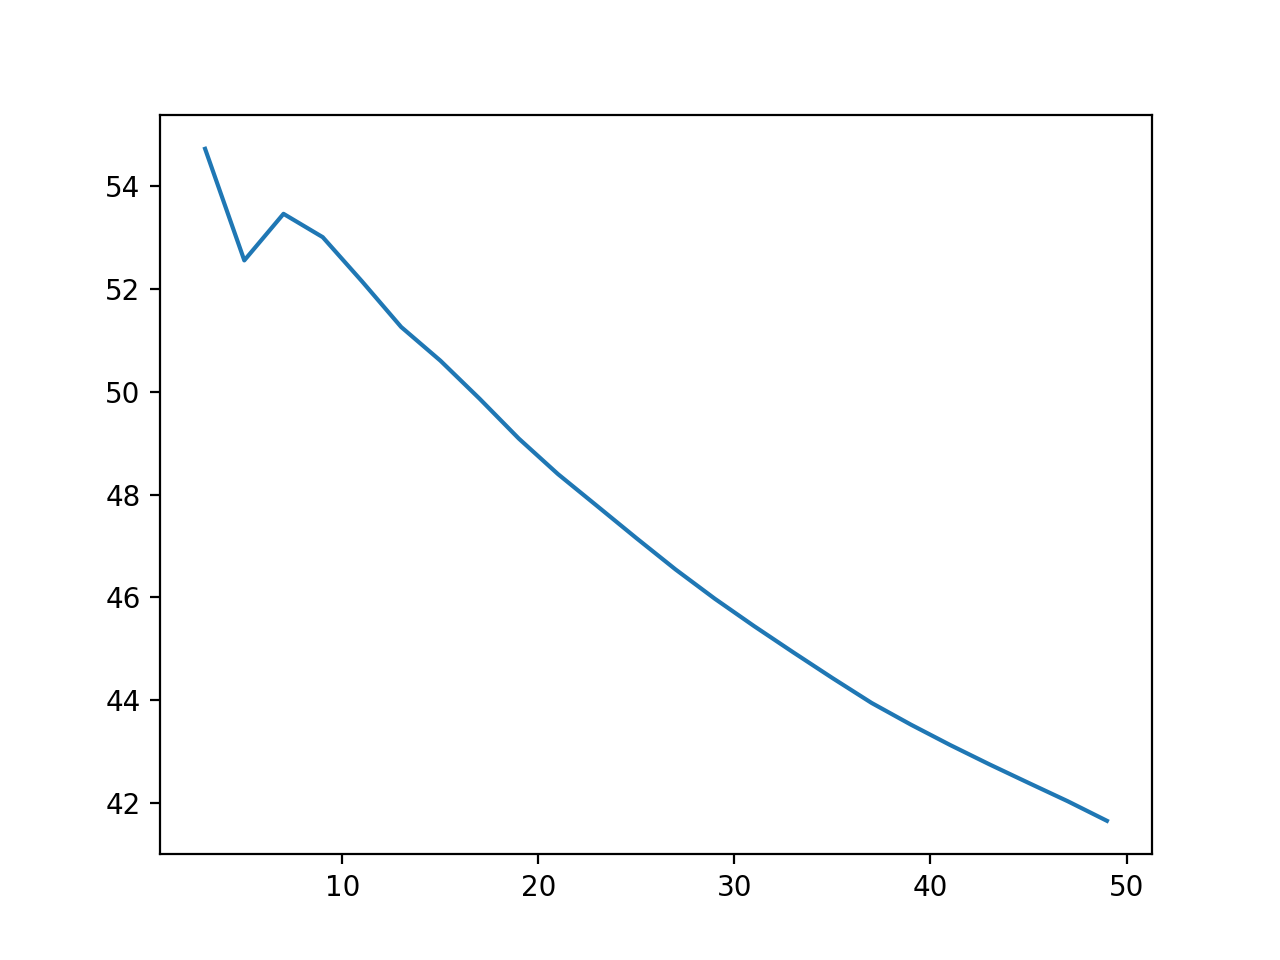
\includegraphics[scale=.45]{./basic_denoising/barbara/median_psnr_sp.png}
      \caption{PSNR vs filter size}
    \endminipage
    \end{figure}
    \pagebreak
% -------------------------------------------------------
% Complete
    
% -------------------------------------------------------
% -------------------------------------------------------
% Boat
% -------------------------------------------------------
% Gaussian
    \subsubsection*{Boat (Gaussian)}
    
%   Image
    \begin{figure}[!htb]
    \begin{center}
     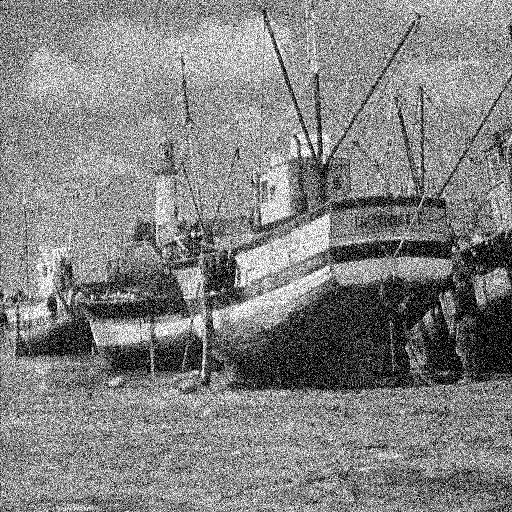
\includegraphics[scale=.3]{./basic_denoising/boat/gaussian.png}
     \caption{Gaussian Noise}
    \end{center}
    \end{figure}
    
%   Mean Filter
    \begin{figure}[!htb]
    \minipage{0.45\textwidth}
      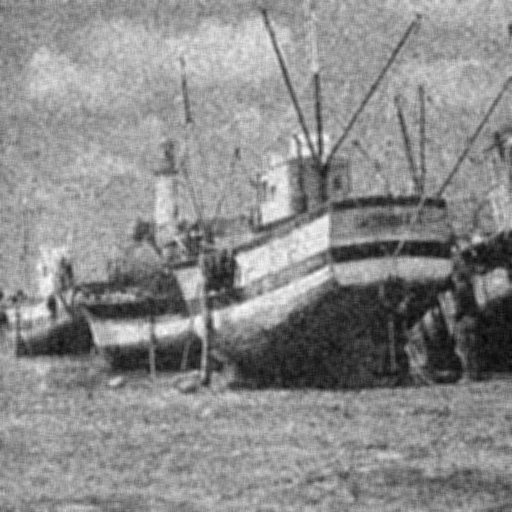
\includegraphics[scale=0.3]{./basic_denoising/boat/average_best_gaussian.png}
      \caption{Best PSNR image}
    \endminipage \hfill
    \minipage{0.45\textwidth}
      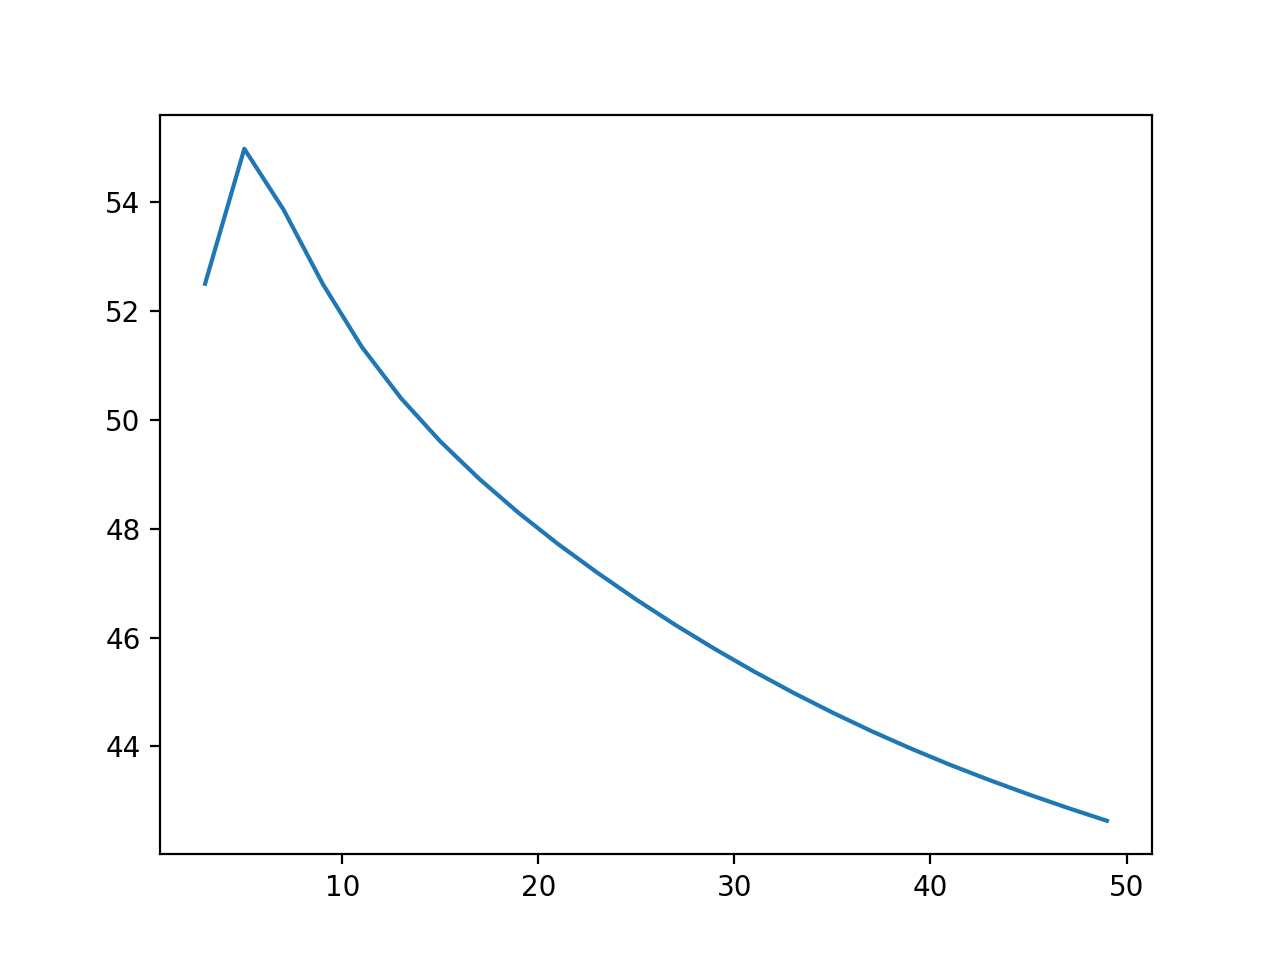
\includegraphics[scale=.45]{./basic_denoising/boat/average_psnr_gaussian.png}
      \caption{PSNR vs filter size}
    \endminipage
    \end{figure}
    
%   Median Filter
    \begin{figure}[!htb]
    \minipage{0.45\textwidth}
      
\includegraphics[scale=0.3]{./basic_denoising/boat/median_best_gaussian.png}
      \caption{Best PSNR image}
    \endminipage \hfill
    \minipage{0.45\textwidth}
      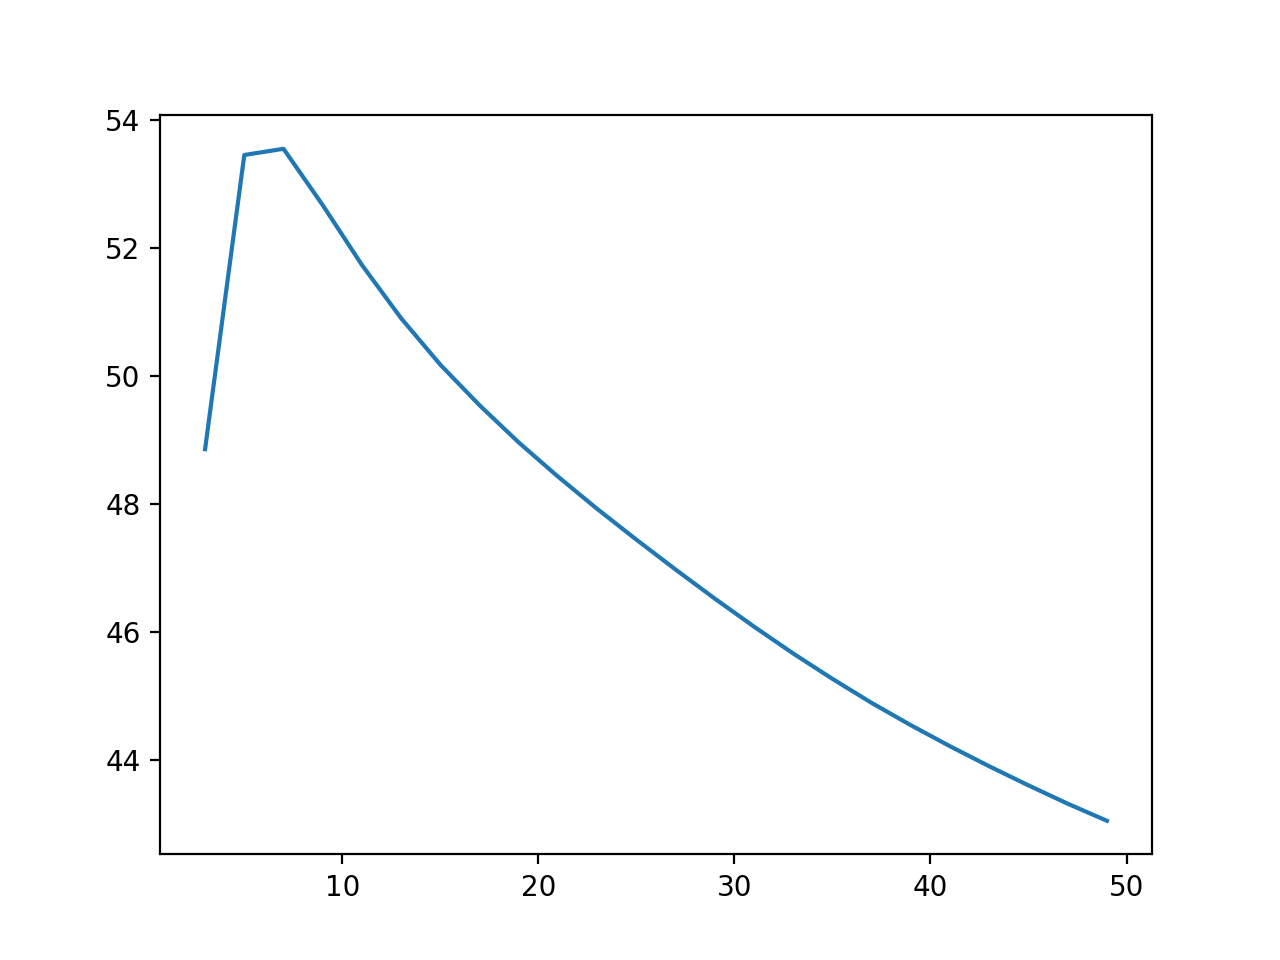
\includegraphics[scale=.45]{./basic_denoising/boat/median_psnr_gaussian.png}
      \caption{PSNR vs filter size}
    \endminipage
    \end{figure}
    \pagebreak
% -------------------------------------------------------
% Salt\Pepper
    \subsubsection*{Boat (Salt/Pepper)}
    
%   Image
    \begin{figure}[!htb]
    \begin{center}
     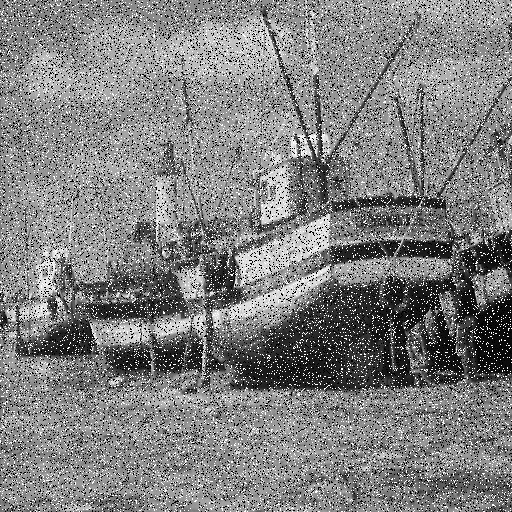
\includegraphics[scale=.3]{./basic_denoising/boat/sp.png}
     \caption{Salt/Pepper Noise}
    \end{center}
    \end{figure}
    
%   Mean Filter
    \begin{figure}[!htb]
    \minipage{0.45\textwidth}
      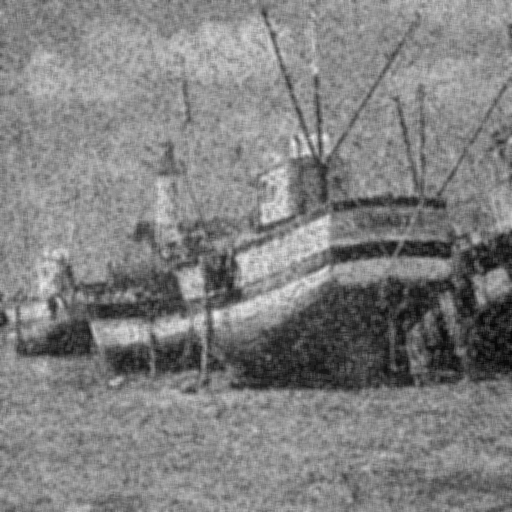
\includegraphics[scale=0.3]{./basic_denoising/boat/average_best_sp.png}
      \caption{Best PSNR image}
    \endminipage \hfill
    \minipage{0.45\textwidth}
      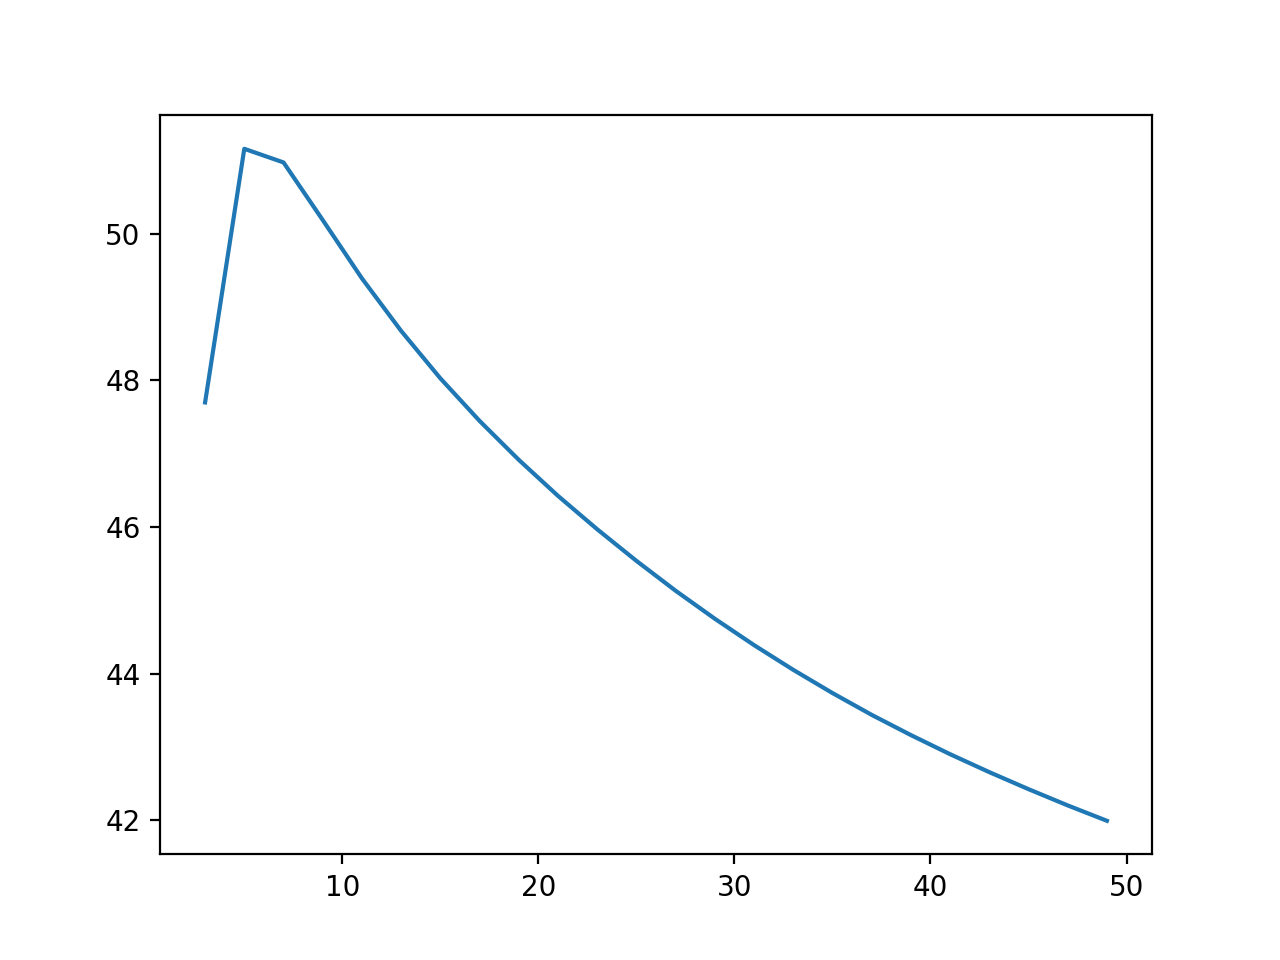
\includegraphics[scale=.45]{./basic_denoising/boat/average_psnr_sp.png}
      \caption{PSNR vs filter size}
    \endminipage
    \end{figure}
    
%   Median Filter
    \begin{figure}[!htb]
    \minipage{0.45\textwidth}
      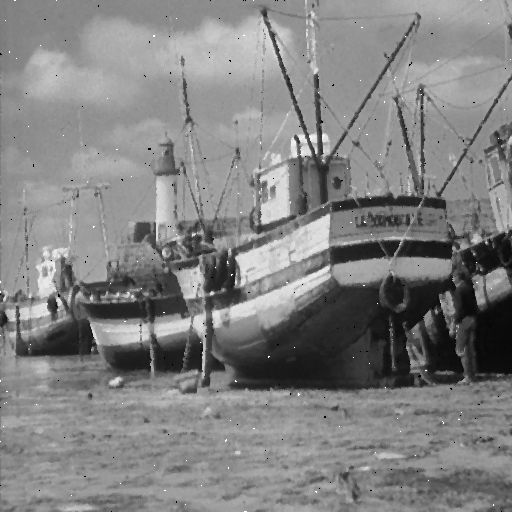
\includegraphics[scale=0.3]{./basic_denoising/boat/median_best_sp.png}
      \caption{Best PSNR image}
    \endminipage \hfill
    \minipage{0.45\textwidth}
      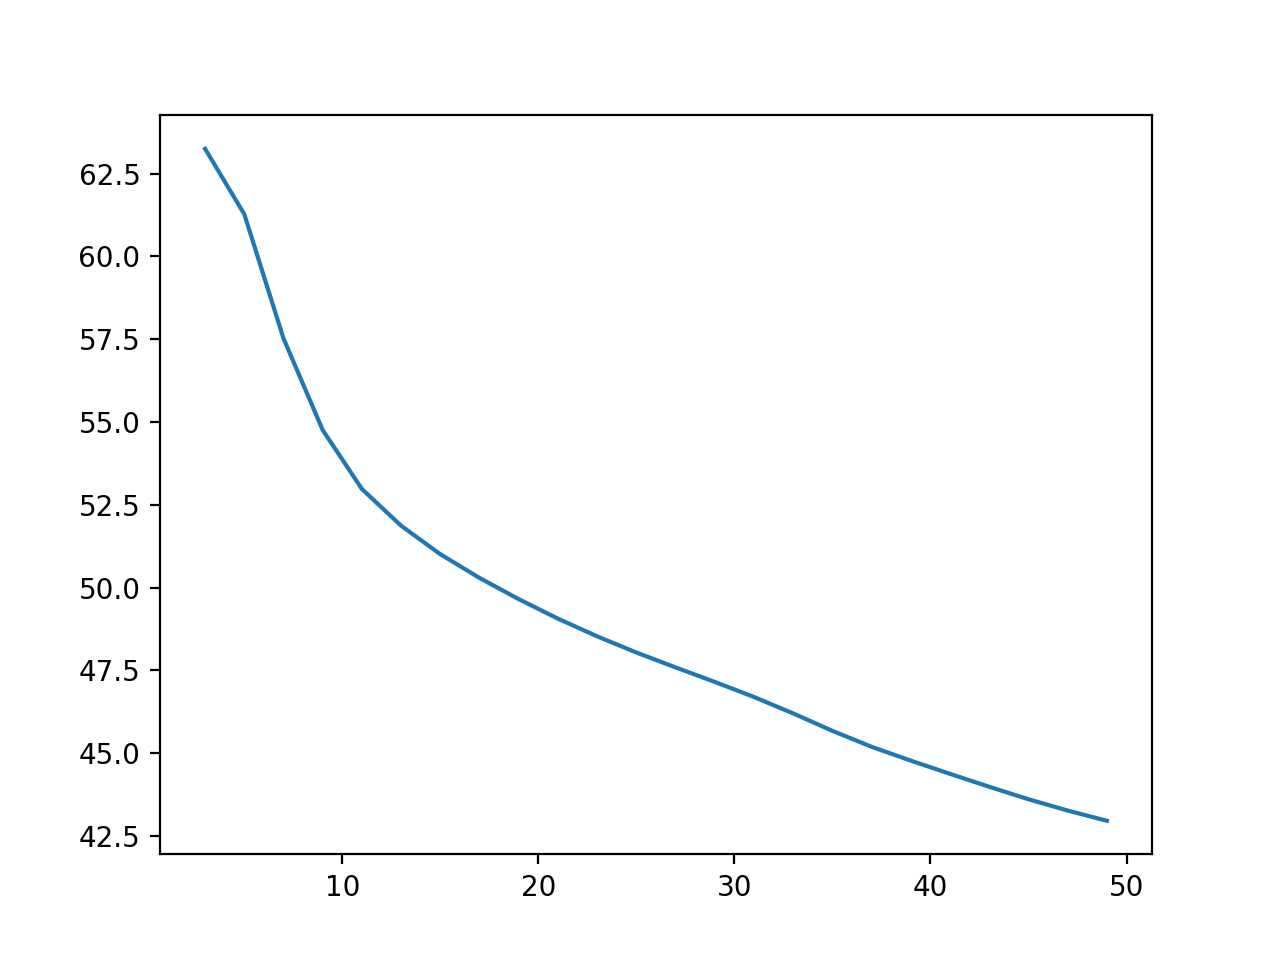
\includegraphics[scale=.45]{./basic_denoising/boat/median_psnr_sp.png}
      \caption{PSNR vs filter size}
    \endminipage
    \end{figure}
    \pagebreak
% -------------------------------------------------------
% Complete

% -------------------------------------------------------
% -------------------------------------------------------
% Sandiego
% -------------------------------------------------------
% Gaussian
    \subsubsection*{Sandiego (Gaussian)}
    
%   Image
    \begin{figure}[!htb]
    \begin{center}
     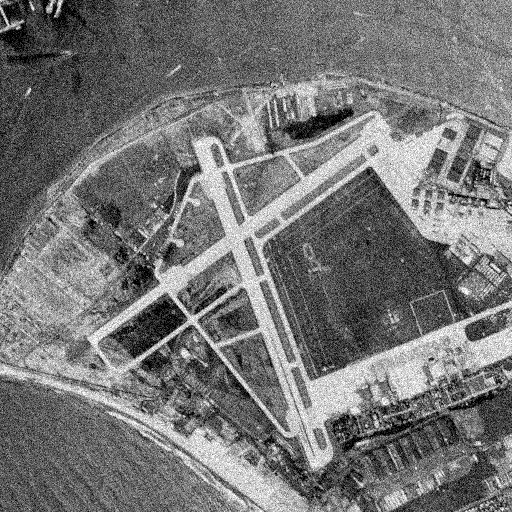
\includegraphics[scale=.3]{./basic_denoising/sandiego/gaussian.png}
     \caption{Gaussian Noise}
    \end{center}
    \end{figure}
    
%   Mean Filter
    \begin{figure}[!htb]
    \minipage{0.45\textwidth}
      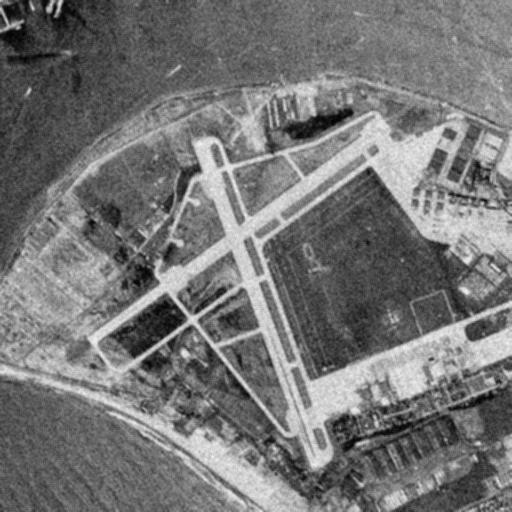
\includegraphics[scale=0.3]{./basic_denoising/sandiego/average_best_gaussian.png}
      \caption{Best PSNR image}
    \endminipage \hfill
    \minipage{0.45\textwidth}
      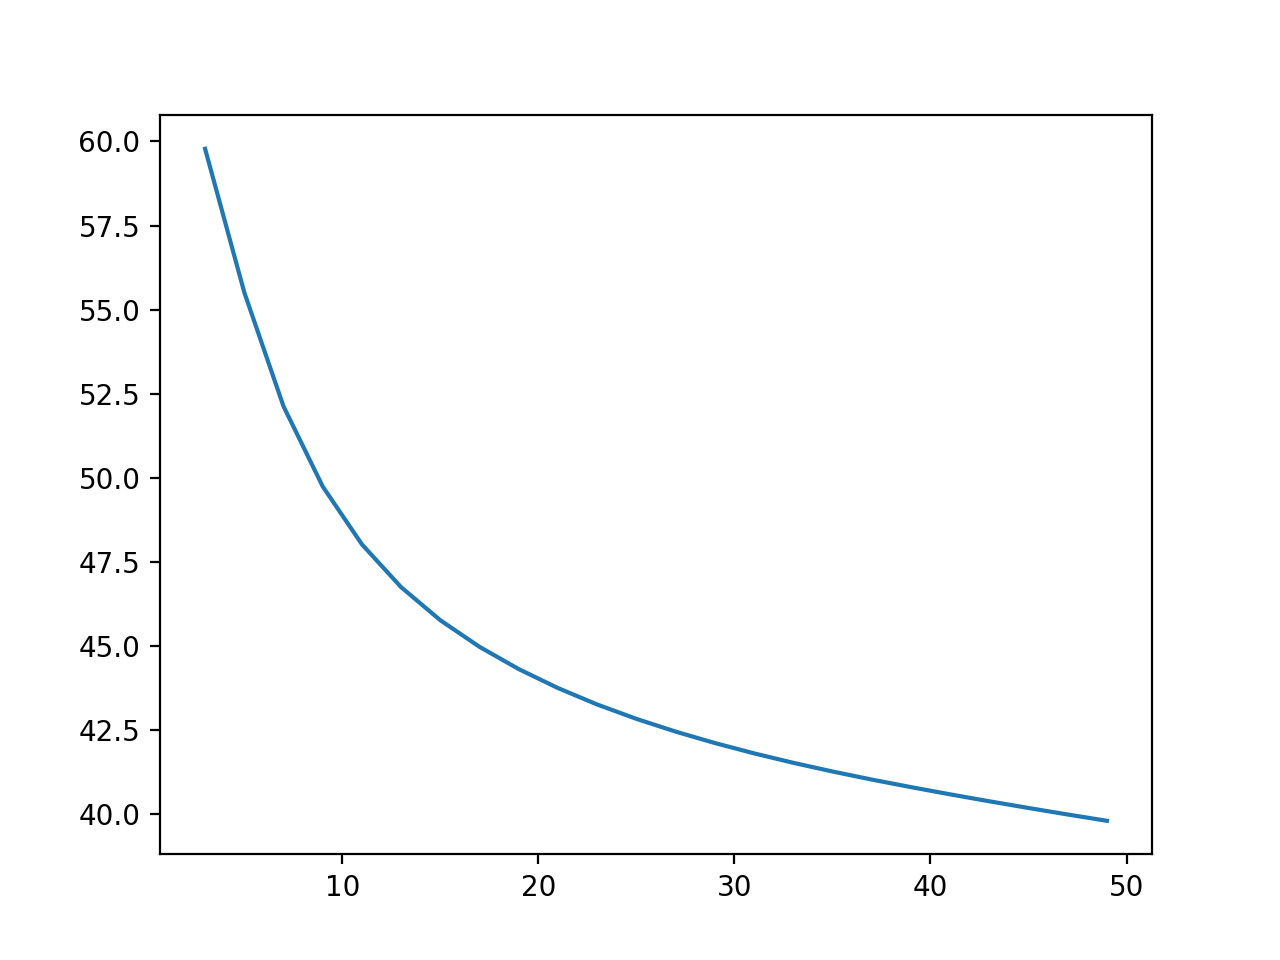
\includegraphics[scale=.45]{./basic_denoising/sandiego/average_psnr_gaussian.png}
      \caption{PSNR vs filter size}
    \endminipage
    \end{figure}
    
%   Median Filter
    \begin{figure}[!htb]
    \minipage{0.45\textwidth}
      
\includegraphics[scale=0.3]{./basic_denoising/sandiego/median_best_gaussian.png}
      \caption{Best PSNR image}
    \endminipage \hfill
    \minipage{0.45\textwidth}
      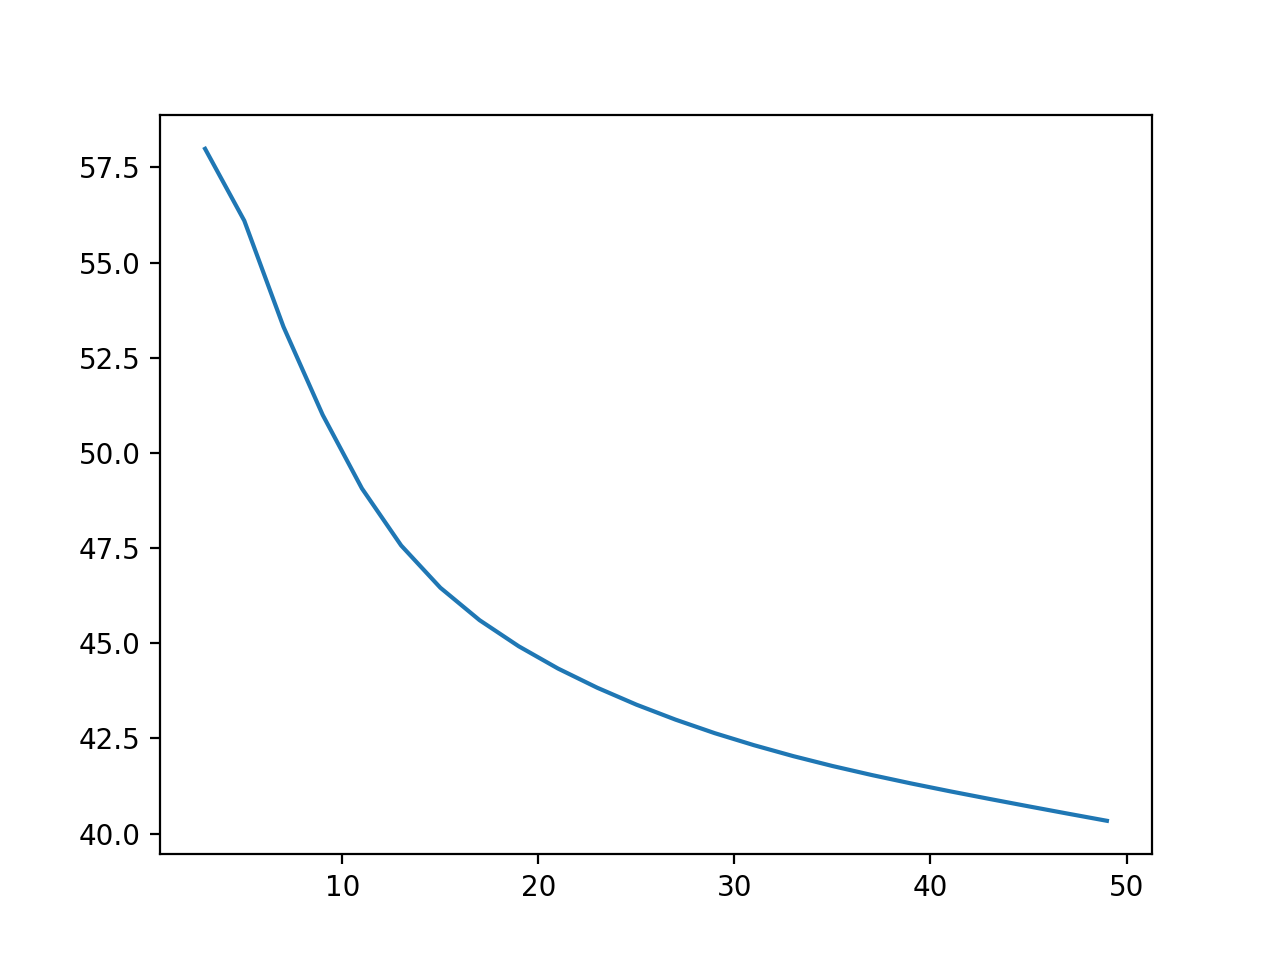
\includegraphics[scale=.45]{./basic_denoising/sandiego/median_psnr_gaussian.png}
      \caption{PSNR vs filter size}
    \endminipage
    \end{figure}
    \pagebreak
% -------------------------------------------------------
% Salt\Pepper
    \subsubsection*{Sandiego (Salt/Pepper)}
    
%   Image
    \begin{figure}[!htb]
    \begin{center}
     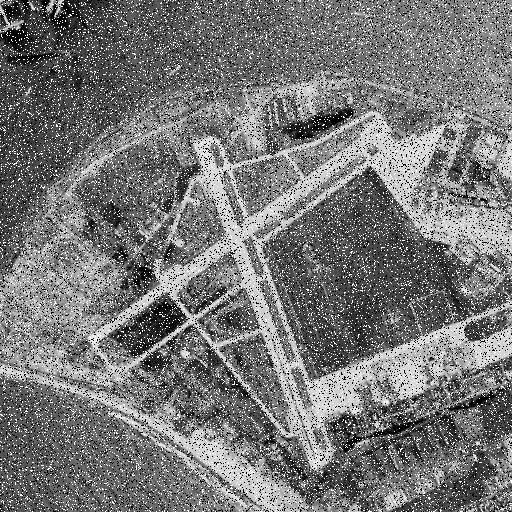
\includegraphics[scale=.3]{./basic_denoising/sandiego/sp.png}
     \caption{Salt/Pepper Noise}
    \end{center}
    \end{figure}
    
%   Mean Filter
    \begin{figure}[!htb]
    \minipage{0.45\textwidth}
      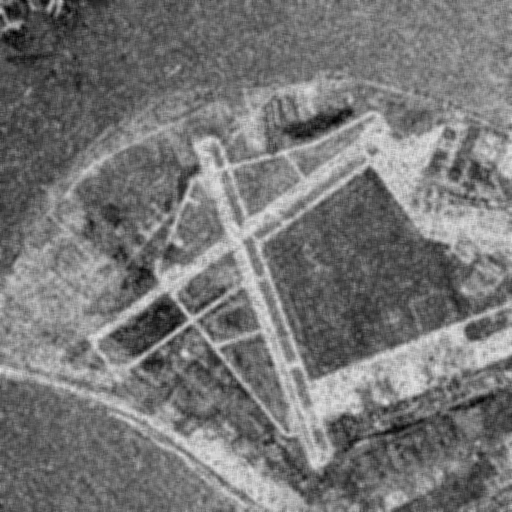
\includegraphics[scale=0.3]{./basic_denoising/sandiego/average_best_sp.png}
      \caption{Best PSNR image}
    \endminipage \hfill
    \minipage{0.45\textwidth}
      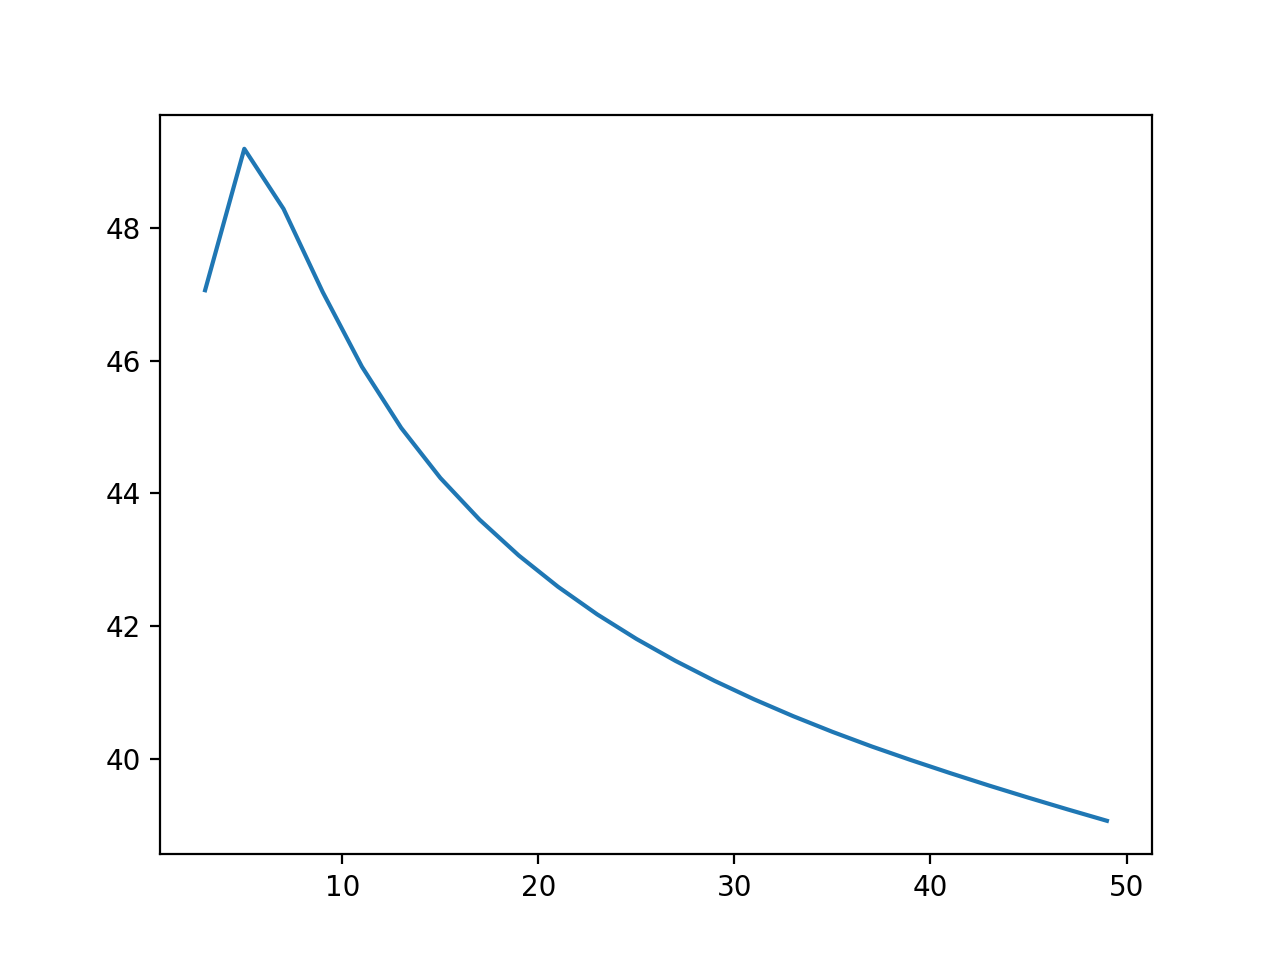
\includegraphics[scale=.45]{./basic_denoising/sandiego/average_psnr_sp.png}
      \caption{PSNR vs filter size}
    \endminipage
    \end{figure}
    
%   Median Filter
    \begin{figure}[!htb]
    \minipage{0.45\textwidth}
      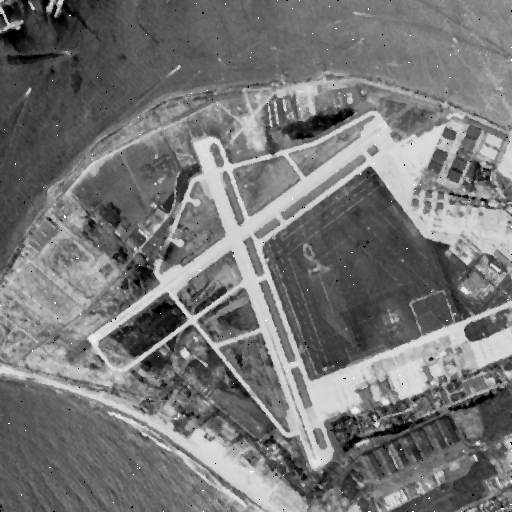
\includegraphics[scale=0.3]{./basic_denoising/sandiego/median_best_sp.png}
      \caption{Best PSNR image}
    \endminipage \hfill
    \minipage{0.45\textwidth}
      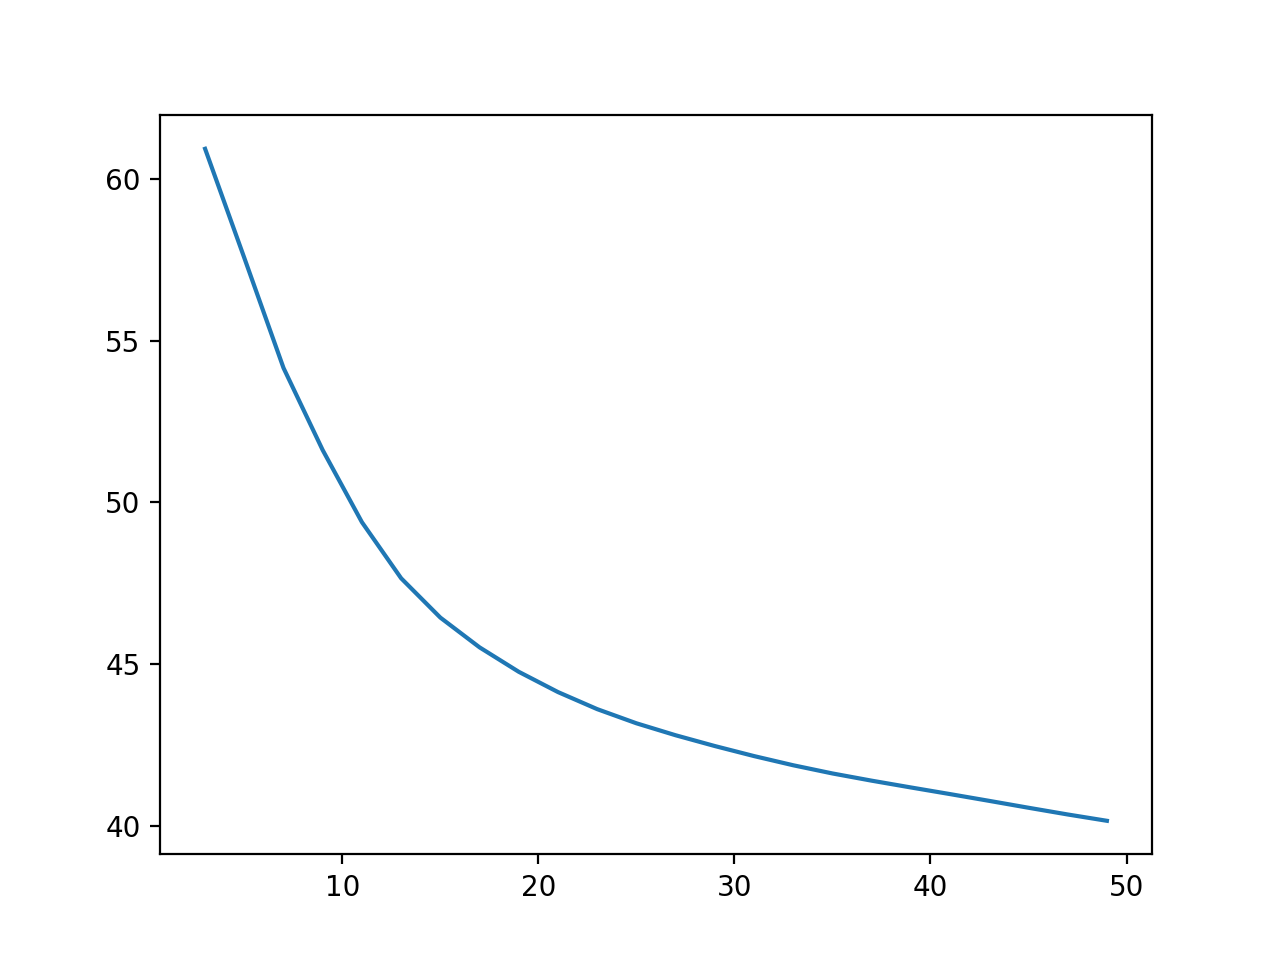
\includegraphics[scale=.45]{./basic_denoising/sandiego/median_psnr_sp.png}
      \caption{PSNR vs filter size}
    \endminipage
    \end{figure}
    \pagebreak
% -------------------------------------------------------
% Complete

% -------------------------------------------------------
% -------------------------------------------------------
% Shepplogan
% -------------------------------------------------------
% Gaussian
    \subsubsection*{Shepplogan (Gaussian)}
    
%   Image
    \begin{figure}[!htb]
    \begin{center}
     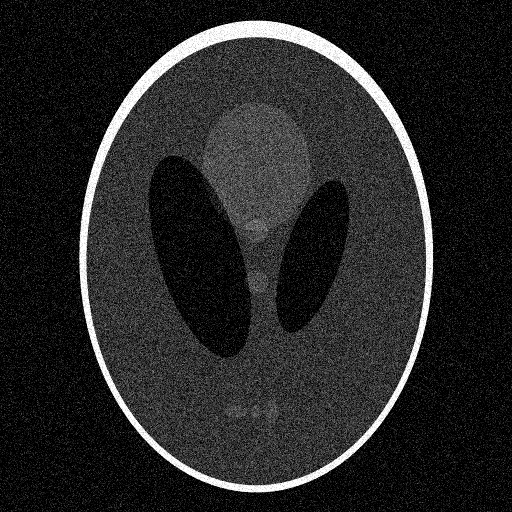
\includegraphics[scale=.3]{./basic_denoising/shepplogan/gaussian.png}
     \caption{Gaussian Noise}
    \end{center}
    \end{figure}
    
%   Mean Filter
    \begin{figure}[!htb]
    \minipage{0.45\textwidth}
      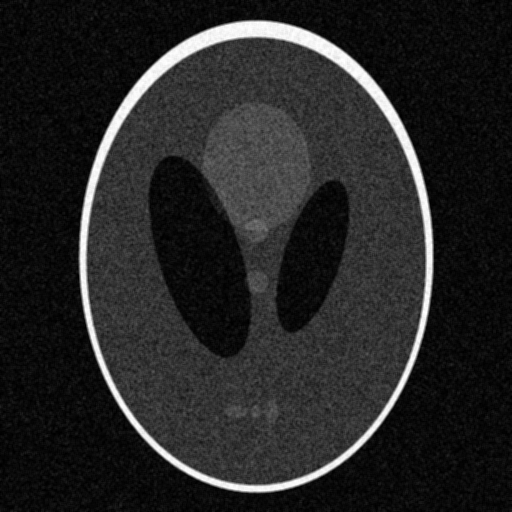
\includegraphics[scale=0.3]{./basic_denoising/shepplogan/average_best_gaussian.png}
      \caption{Best PSNR image}
    \endminipage \hfill
    \minipage{0.45\textwidth}
      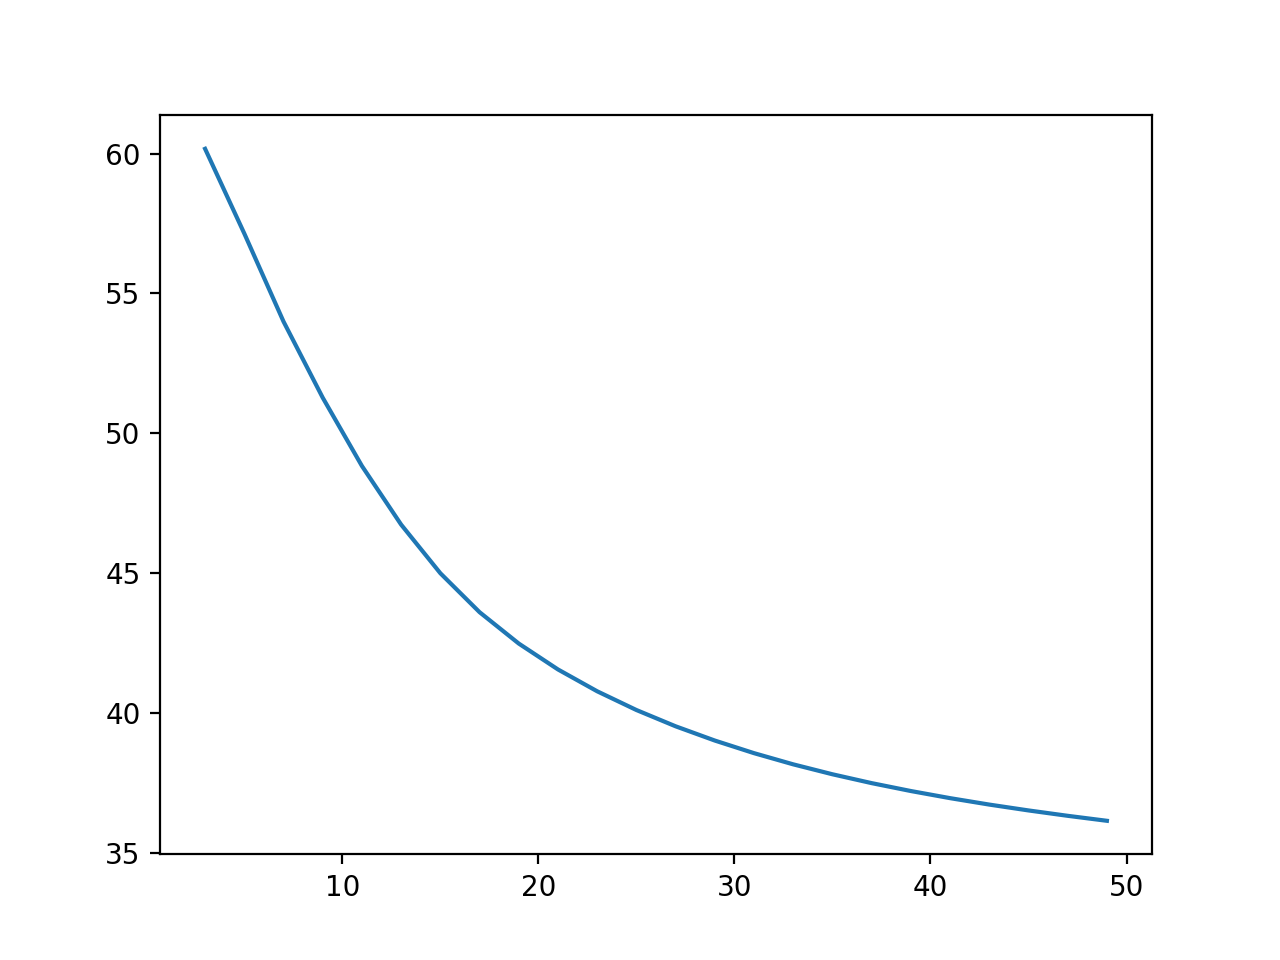
\includegraphics[scale=.45]{./basic_denoising/shepplogan/average_psnr_gaussian.png}
      \caption{PSNR vs filter size}
    \endminipage
    \end{figure}
    
%   Median Filter
    \begin{figure}[!htb]
    \minipage{0.45\textwidth}
      
\includegraphics[scale=0.3]{./basic_denoising/shepplogan/median_best_gaussian.png}
      \caption{Best PSNR image}
    \endminipage \hfill
    \minipage{0.45\textwidth}
      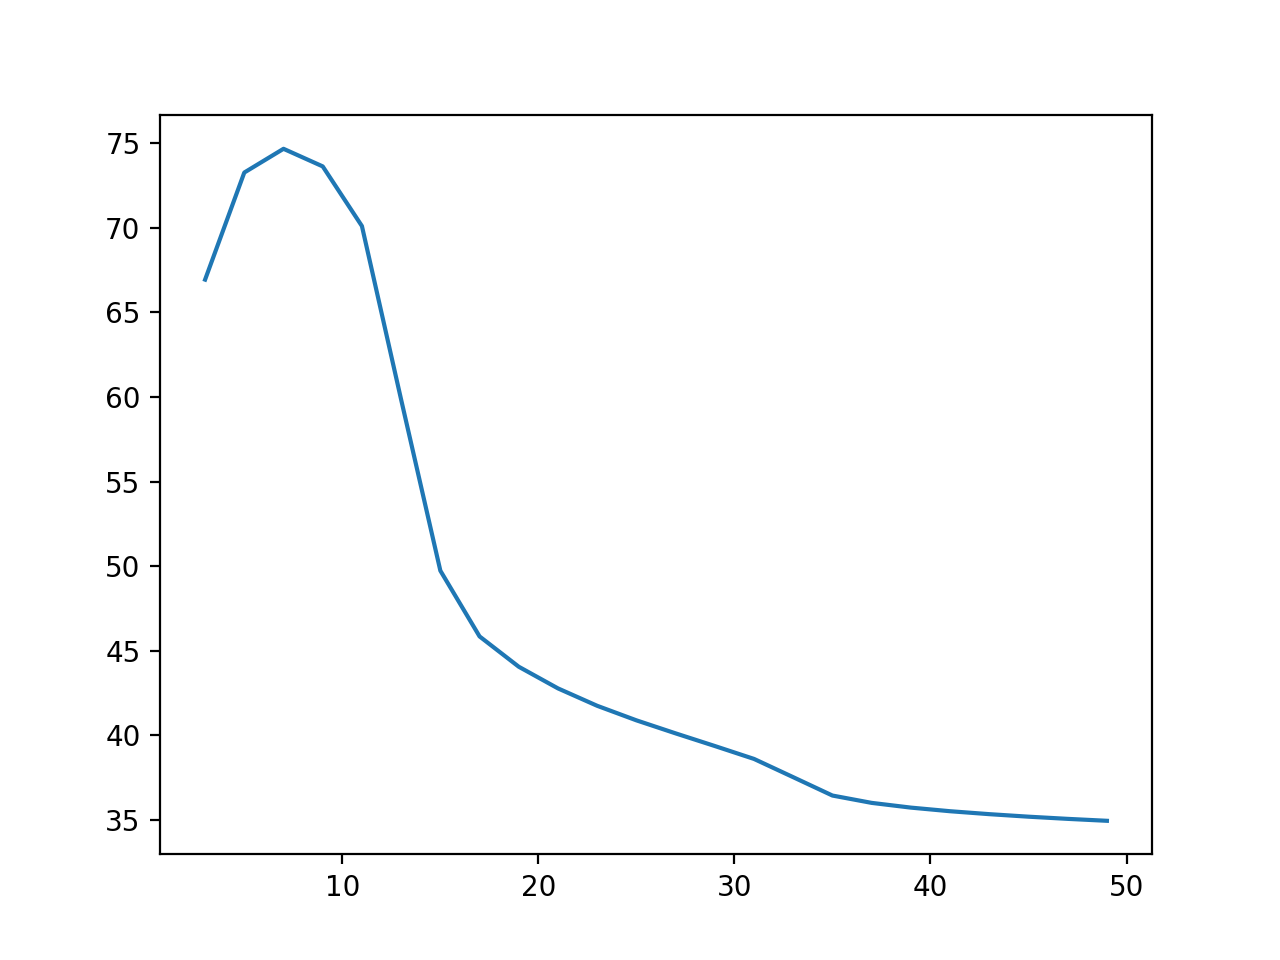
\includegraphics[scale=.45]{./basic_denoising/shepplogan/median_psnr_gaussian.png}
      \caption{PSNR vs filter size}
    \endminipage
    \end{figure}
    \pagebreak
% -------------------------------------------------------
% Salt\Pepper
    \subsubsection*{Shepplogan (Salt/Pepper)}
    
%   Image
    \begin{figure}[!htb]
    \begin{center}
     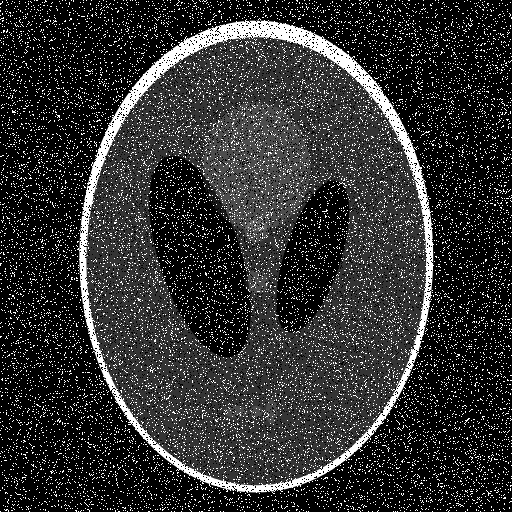
\includegraphics[scale=.3]{./basic_denoising/shepplogan/sp.png}
     \caption{Salt/Pepper Noise}
    \end{center}
    \end{figure}
    
%   Mean Filter
    \begin{figure}[!htb]
    \minipage{0.45\textwidth}
      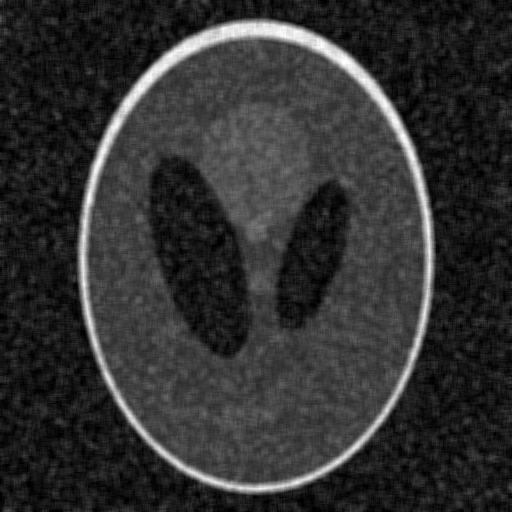
\includegraphics[scale=0.3]{./basic_denoising/shepplogan/average_best_sp.png}
      \caption{Best PSNR image}
    \endminipage \hfill
    \minipage{0.45\textwidth}
      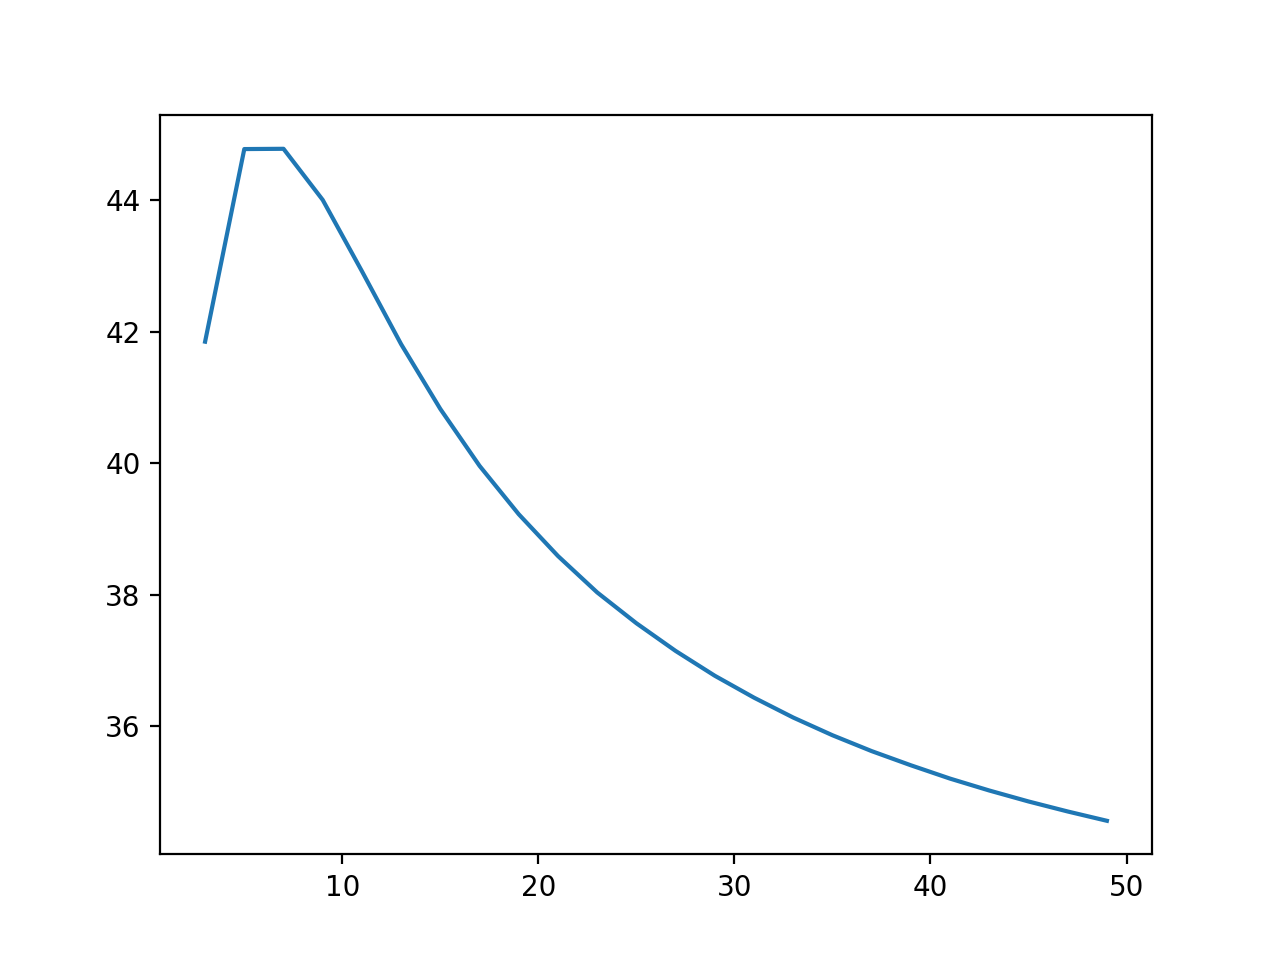
\includegraphics[scale=.45]{./basic_denoising/shepplogan/average_psnr_sp.png}
      \caption{PSNR vs filter size}
    \endminipage
    \end{figure}
    
%   Median Filter
    \begin{figure}[!htb]
    \minipage{0.45\textwidth}
      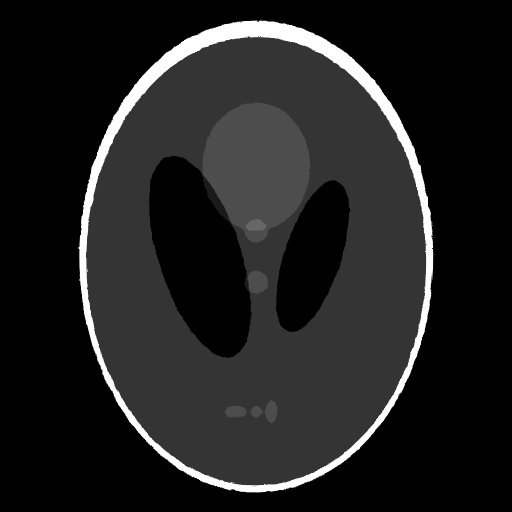
\includegraphics[scale=0.3]{./basic_denoising/shepplogan/median_best_sp.png}
      \caption{Best PSNR image}
    \endminipage \hfill
    \minipage{0.45\textwidth}
      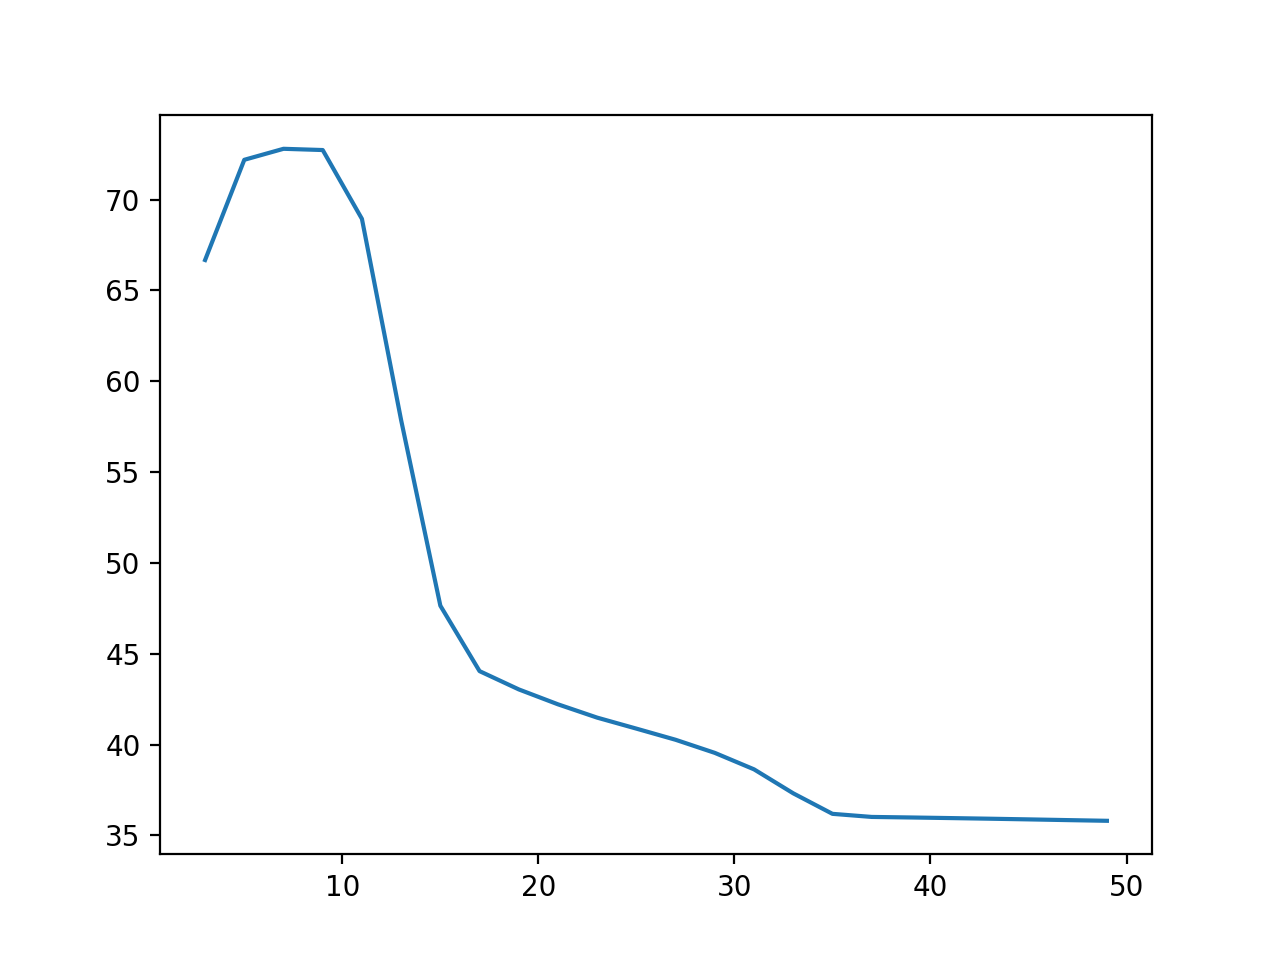
\includegraphics[scale=.45]{./basic_denoising/shepplogan/median_psnr_sp.png}
      \caption{PSNR vs filter size}
    \endminipage
    \end{figure}
    \pagebreak
% -------------------------------------------------------
% Complete

    
% -------------------------------------------------------
% -------------------------------------------------------
% Topic I
    \pagebreak
    \subsection*{Edge-Perserving Smoothing}
    I implemented the \textit{total variation denoising} and used it on the images from previous discussion. Also, followed are results from an example implementation of total variation.
    
    \begin{figure}[!htb]
    \minipage{0.45\textwidth}
      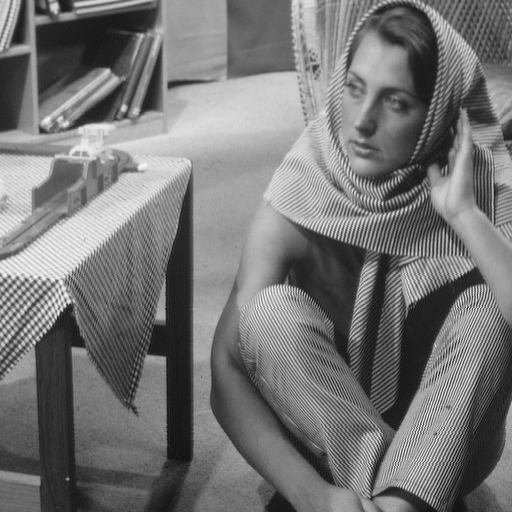
\includegraphics[scale=.35]{../images/barbara.png}
      \caption{Barbara}
    \endminipage \hfill
    \minipage{0.45\textwidth}
      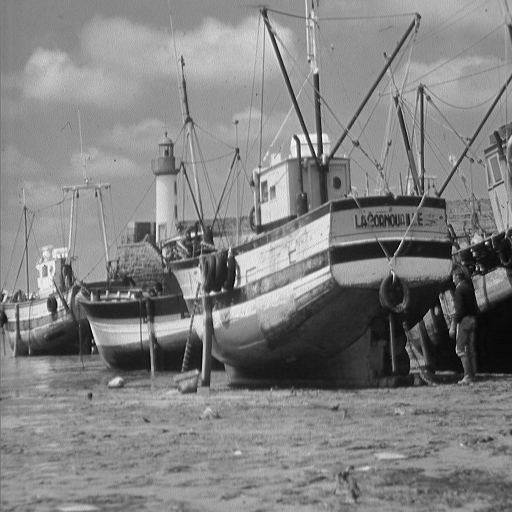
\includegraphics[scale=1.55]{../images/boat.png}
      \caption{Boat}
    \endminipage
    \end{figure}
    
    \phantom{}
    
    \begin{figure}[!htb]
    \minipage{0.45\textwidth}
      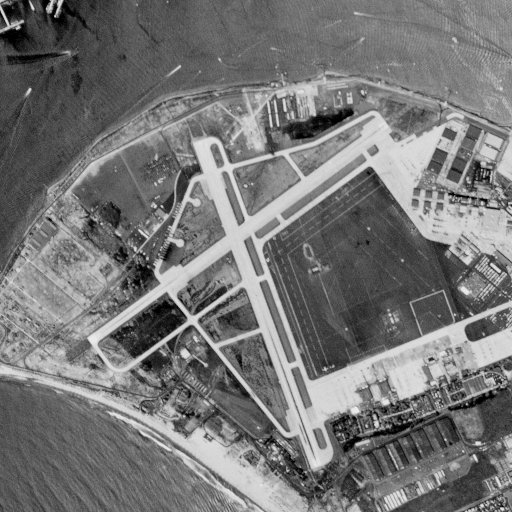
\includegraphics[scale=1.4]{../images/sandiego.png}
      \caption{Sandiego}
    \endminipage \hfill
    \minipage{0.45\textwidth}
      
\includegraphics[scale=.35]{../images/shepplogan.png}
      \caption{Shepplogan}
    \endminipage
    \end{figure}
    \pagebreak
% -------------------------------------------------------
% Complete

    
    \subsection*{Tone Mapping Algorithm}
    In this section, I focused on implementing the \textbf{Reinhard Tone Map} and applied on a set of images. The original images produced, were processed to give promising mappings, shown below.
    \begin{center}
        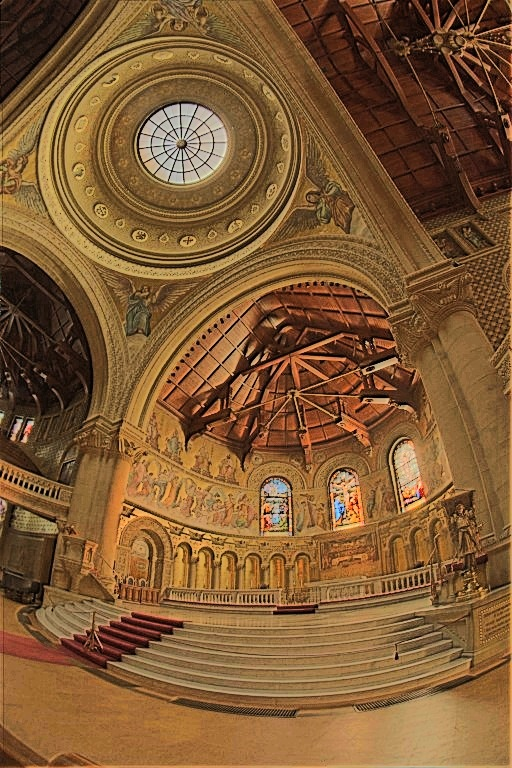
\includegraphics[scale=.27]{./data/3/fnl.jpg}
    \end{center}
    Also, following was the general variation in the deciding s parameter.
    \begin{center}
        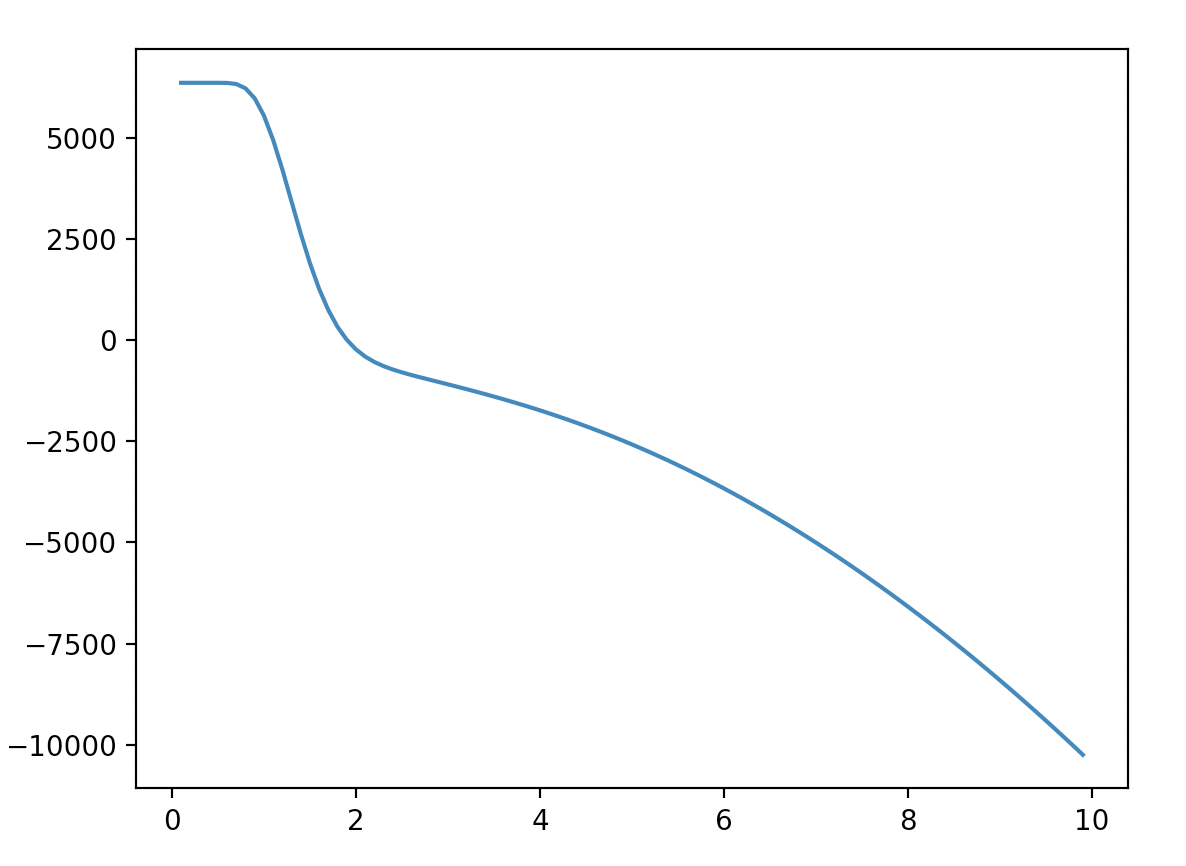
\includegraphics[scale=.27]{./data/3/plot.png}
    \end{center}
    \pagebreak
    Also, following are how images vary if different parameters are set.
    \begin{figure}[!htb]
    \minipage{0.32\textwidth}
      \includegraphics[scale=.27]{./data/3/svar/s1.jpg}
      \caption{s = 0.1}
    \endminipage\hfill
    \minipage{0.32\textwidth}
      \includegraphics[scale=.27]{./data/3/svar/s2.jpg}
      \caption{s = 2.1 (Optimal)}
    \endminipage\hfill
    \minipage{0.32\textwidth}%
      \includegraphics[scale=.27]{./data/3/svar/s3.jpg}
      \caption{s = 9.9}
    \endminipage
    \end{figure}
    \begin{figure}[!htb]
    \minipage{0.32\textwidth}
      \includegraphics[scale=.27]{./data/3/avar/3_6.jpg}
      \caption{key = .36}
    \endminipage\hfill
    \minipage{0.32\textwidth}
      \includegraphics[scale=.27]{./data/3/avar/4_5.jpg}
      \caption{key = .45}
    \endminipage\hfill
    \minipage{0.32\textwidth}%
      \includegraphics[scale=.27]{./data/3/avar/7_2.jpg}
      \caption{key = .72}
    \endminipage
    \end{figure}
    \\
    \pagebreak
    \\
    The results from the tonemapping algorithm are distinctively better than the methods implemented before. Seemingly intelligent, the tone-map provides gives a more realistic idea of how the original image may have looked. \\
    \subsection*{Summary}
    All required by the assignment was implemented and a lot of new things were learned/understood. The codes are written in Python (for part 1 \& 3) and in C++ (for part 2). All the functions were implemented on own (except for the FFT, which was allowed to be used). \\
    I am also looking forward to implementing other options from the assignment (which unfortunately due to internship acquiring process I couldn't devote time to).\\
    The assignment was intriguing and I learnt a lot of new ideas. Thanks and Regards.
    
\end{document}